\chapter{ऐल्कीनों का ऑक्सीकरण और अपचयन}\label{ch:b2:alkene-redox}

दो-भाग वाला एपॉक्सी गोंद दो ट्यूबों में आता है: एक में ऐसे अणु होते हैं जिनके सिरों पर
\omterm{def:b2:alkene-redox:epoxide}{एपॉक्साइड} वलय हैं, अर्थात् दो कार्बनों और एक ऑक्सीजन के त्रिसदस्यी वलय; दूसरे में एक
ऐमीन। मिलाने पर तनावग्रस्त वलय एक के बाद एक खुलते हैं और लेप कठोर
जाल में जम जाता है। ऐल्कीन ऐसे वलयों के कच्चे माल हैं, उन ऐल्कोहॉलों के भी जो
वहाँ लगते हैं जहाँ मार्कोवनिकोव का नियम उन्हें कभी न रखता, चुनी हुई ज्यामिति वाले
डाइऑलों के भी, और उन छोटे खंडों के भी जिनसे कभी रसायनज्ञ जानते थे कि किसी अणु में द्वि-आबंध
कहाँ था। यह अध्याय प्रथम वर्ष के खंड के इलेक्ट्रॉनरागी योगों में
वे अभिक्रियाएँ जोड़ता है जो द्वि-आबंध का अपचयन या ऑक्सीकरण करती हैं, और
उनमें से हर एक द्वारा थोपा गया त्रिविम-रसायन भी।

\begin{recall}
प्रथम वर्ष का खंड: इलेक्ट्रॉनरागी योग, मार्कोवनिकोव का नियम, हैलोनियम आयन,
सम-योग और प्रति-योग, ऐल्कीनों का जलयोजन, कार्बन के ऑक्सीकरण स्तर,
हाइड्राइड दाता, रसायनवरणात्मकता, मेसो यौगिक और रेसेमिक मिश्रण,
त्रिविमविशिष्ट अभिक्रियाएँ। \Cref{ch:b2:catalytic-cycles}:
विल्किन्सन उत्प्रेरक का हाइड्रोजनन चक्र।
\end{recall}

\begin{omfigure}
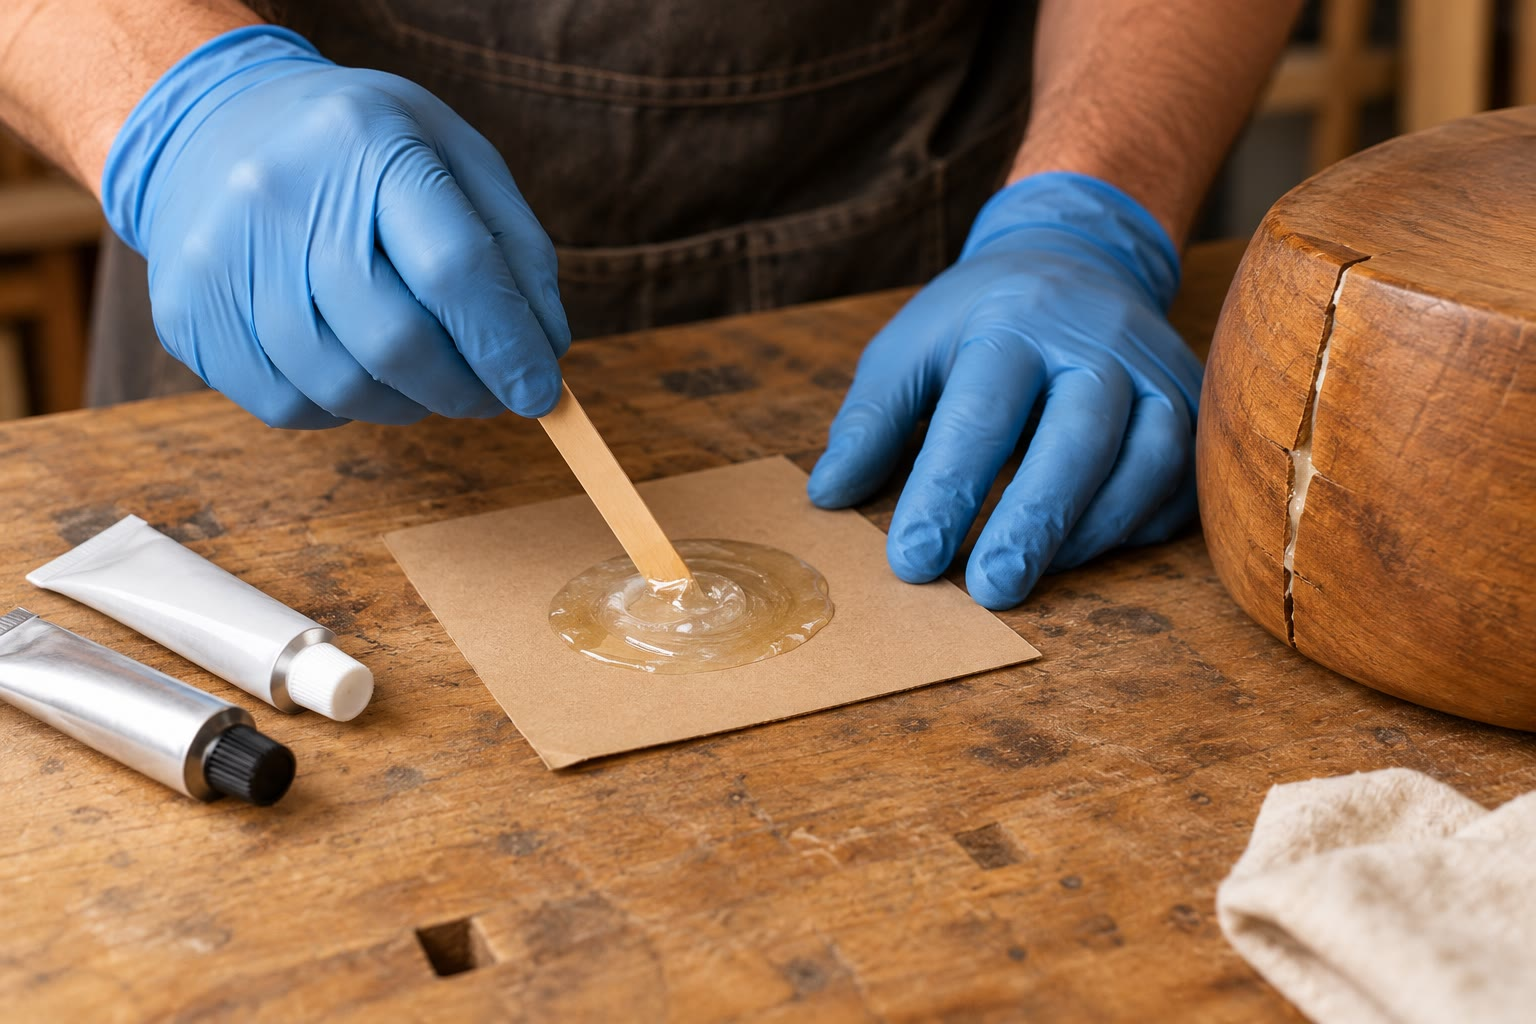
\includegraphics[width=0.6\linewidth]{images/book3/ai/b2-21-epoxy.jpg}

{\small दो-भाग वाले एपॉक्सी गोंद को मिलाना: रेज़िन, जिसमें \omterm{def:b2:alkene-redox:epoxide}{एपॉक्साइड} समूह हैं, और
कठोरक, एक ऐमीन, मिलते ही अभिक्रिया करते हैं; वलय खुलते हैं और अणुओं को
एक ठोस जाल में जोड़ देते हैं।}
\end{omfigure}

\section{उत्प्रेरकी हाइड्रोजनन}

\begin{definition}[उत्प्रेरकी हाइड्रोजनन]\label{def:b2:alkene-redox:hydrogenation}
\emph{उत्प्रेरकी हाइड्रोजनन}\index{उत्प्रेरकी हाइड्रोजनन} किसी उत्प्रेरक की उपस्थिति में किसी
बहु-आबंध पर डाइहाइड्रोजन जोड़ता है: विषमांगी उत्प्रेरण में कोई सूक्ष्म-विभाजित धातु (कार्बन पर
पैलेडियम, प्लैटिनम, निकेल), या समांगी उत्प्रेरण में विल्किन्सन
उत्प्रेरक जैसा कोई विलेय संकुल।
\end{definition}

किसी धातु सतह पर डाइहाइड्रोजन और ऐल्कीन दोनों पकड़े जाते हैं, \ce{H-H} आबंध
सतही हाइड्रोजन परमाणुओं में टूट जाता है, और ये एक के बाद एक ऐल्कीन के कार्बन
परमाणुओं पर स्थानांतरित होते हैं, जो धातु पर सपाट पड़ी होती है।

\begin{proposition}[सम-योग]\label{prop:b2:alkene-redox:syn-hydrogenation}
\omterm{def:b2:alkene-redox:hydrogenation}{उत्प्रेरकी हाइड्रोजनन} दोनों हाइड्रोजन परमाणुओं को द्वि-आबंध के एक ही फलक पर पहुँचाता है।
विषाक्त पैलेडियम उत्प्रेरक पर हाइड्रोजनित कोई ऐल्काइन ऐल्कीन पर रुक जाती है, जो
(\textit{Z}) समावयवी होती है।
\end{proposition}

\begin{proof}[तर्क]
ऐल्कीन उत्प्रेरक से अपने एक फलक द्वारा बँधी होती है, और दोनों हाइड्रोजन उत्प्रेरक से,
उसी फलक पर, आते हैं: सम-योग। किसी ऐल्काइन के साथ त्रि-आबंध पर जोड़े गए दोनों हाइड्रोजन
एक ही ओर, एक-दूसरे के cis, होते हैं: (\textit{Z})-ऐल्कीन। आंशिक रूप से
निष्क्रियित उत्प्रेरक (लेड लवण और क्विनोलीन के साथ कैल्सियम कार्बोनेट पर पैलेडियम)
ऐल्काइन को बनी हुई ऐल्कीन की तुलना में कहीं अधिक प्रबलता से बाँधता है, और वह ऐल्कीन
दूसरे योग से पहले सतह छोड़ देती है।
\end{proof}

\section{हाइड्रोबोरॉनन--ऑक्सीकरण}

\begin{definition}[हाइड्रोबोरॉनन]\label{def:b2:alkene-redox:hydroboration}
\emph{हाइड्रोबोरॉनन}\index{हाइड्रोबोरॉनन} किसी बोरेन का एक B--H आबंध किसी
\ce{C=C} आबंध पर जोड़ता है; क्षारीय हाइड्रोजन परॉक्साइड से ऑक्सीकरण के बाद यह
ऐल्कीन को ऐसे ऐल्कोहॉल में बदलता है जिसका हाइड्रॉक्सिल समूह कम प्रतिस्थापित कार्बन पर होता है:
\emph{प्रति-मार्कोवनिकोव अभिविन्यास}\index{प्रति-मार्कोवनिकोव अभिविन्यास}।
\end{definition}
\begin{omfigure}
\setchemfig{atom sep=1.8em}
\schemestart[][west]
\chemfig{H_3C-[:30]CH=[:-30]CH_2}
\+ \chemfig{H-BH_2}
\arrow{->[सम-योग]}
\chemfig{H_3C-[:30]CH_2-[:-30]CH_2-[:30]BH_2}
\arrow{->[\ce{H2O2}][\ce{HO-}]}
\chemfig{H_3C-[:30]CH_2-[:-30]CH_2-[:30]OH}
\schemestop
\par\vspace{6pt}

{\small प्रोपीन का हाइड्रोबोरॉनन--ऑक्सीकरण। बोरेन एक चरण में जुड़ता है, बोरॉन
अंतस्थ कार्बन पर और हाइड्रोजन भीतरी कार्बन पर, दोनों एक ही फलक पर; ऑक्सीकरण
बोरॉन को \ce{OH} से विन्यास के धारण के साथ प्रतिस्थापित करता है। प्रोपेन-1-ऑल बनता है, न कि
अम्ल-उत्प्रेरित जलयोजन वाला प्रोपेन-2-ऑल।}
\end{omfigure}

\begin{proposition}[हाइड्रोबोरॉनन का अभिविन्यास]\label{prop:b2:alkene-redox:hydroboration-regio}
बोरॉन द्वि-आबंध के कम प्रतिस्थापित कार्बन पर जुड़ता है, और हाइड्रोजन अधिक
प्रतिस्थापित पर; योग सम है।
\end{proposition}

\begin{proof}[तर्क]
खाली p कक्षक वाला बोरॉन इलेक्ट्रॉनरागी है: चतुःकेंद्रीय संक्रमण अवस्था में
(दोनों कार्बन, बोरॉन और हाइड्रोजन) बोरॉन से आबंध C--H आबंध से थोड़ा पहले बनता है, और
दूसरे कार्बन पर एक आंशिक धनात्मक आवेश विकसित होता है, जिसे अधिक
प्रतिस्थापित कार्बन बेहतर वहन करता है; भारी-भरकम बोरॉन समूह भी कम बाधित सिरे को वरीयता देता है। दोनों नए आबंध
एक ही फलक पर, एक समन्वित चरण में, बनते हैं: सम।
\end{proof}

\begin{proposition}[धारण के साथ ऑक्सीकरण]\label{prop:b2:alkene-redox:retention}
क्षारीय हाइड्रोजन परॉक्साइड द्वारा किसी ऐल्किलबोरेन का ऑक्सीकरण हर C--B आबंध को
कार्बन--हाइड्रॉक्सिल आबंध से प्रतिस्थापित करता है, कार्बन पर विन्यास के धारण के साथ।
\end{proposition}

\begin{proof}[तर्क]
हाइड्रोपरॉक्साइड ऋणायन बोरॉन से जुड़ता है; फिर कोई ऐल्किल समूह अपने इलेक्ट्रॉन युग्म के साथ
बोरॉन से सन्निकट ऑक्सीजन पर प्रवास करता है, जबकि हाइड्रॉक्साइड निकलता है; पूरे समय कार्बन अपने आबंध
एक ही ओर रखता है। B--O आबंध का जल-अपघटन ऐल्कोहॉल को मुक्त करता है।
\end{proof}

\section{एपॉक्साइड}

\begin{definition}[एपॉक्साइड]\label{def:b2:alkene-redox:epoxide}
\emph{एपॉक्साइड}\index{एपॉक्साइड} (ऑक्सिरेन) एक चक्रीय ईथर है जिसका वलय त्रिसदस्यी है,
दो कार्बनों और एक ऑक्सीजन का। \emph{एपॉक्सीकरण}\index{एपॉक्सीकरण} किसी ऐल्कीन को
एपॉक्साइड में बदलता है, प्रायः किसी \emph{परॉक्सी अम्ल}\index{परॉक्सी अम्ल} \ce{RCO3H} से, जो
एक ऑक्सीजन परमाणु द्वि-आबंध पर स्थानांतरित करता है।
\end{definition}

\begin{omfigure}
\setchemfig{atom sep=2em}
\schemestart
\chemfig{R-[:30]CH=[:-30]CH-[:30]R}
\+ \chemfig{Ar-C(=[2]O)-O-O-H}
\arrow{->}
\chemfig{[:-60]CH(-[:210]R)*3(-CH(-[:-30]R)-O-)}
\+ \chemfig{Ar-C(=[2]O)-OH}
\schemestop
\par\vspace{6pt}

{\small \omterm{def:b2:alkene-redox:epoxide}{परॉक्सी अम्ल} द्वारा \omterm{def:b2:alkene-redox:epoxide}{एपॉक्सीकरण} (Ar: उदाहरण के लिए एक 3-क्लोरोफ़ेनिल समूह)। \omterm{def:b2:alkene-redox:epoxide}{परॉक्सी अम्ल} का
अंतस्थ ऑक्सीजन एक चरण में द्वि-आबंध पर स्थानांतरित होता है, और दोनों C--O आबंध
एक ही फलक पर बनते हैं।}
\end{omfigure}

\begin{proposition}[त्रिविमविशिष्ट एपॉक्सीकरण]\label{prop:b2:alkene-redox:epoxidation}
\omterm{def:b2:alkene-redox:epoxide}{परॉक्सी अम्ल} द्वारा \omterm{def:b2:alkene-redox:epoxide}{एपॉक्सीकरण} त्रिविमविशिष्ट है: (\textit{Z})-ऐल्कीन cis \omterm{def:b2:alkene-redox:epoxide}{एपॉक्साइड} देती है,
(\textit{E})-ऐल्कीन trans \omterm{def:b2:alkene-redox:epoxide}{एपॉक्साइड}।
\end{proposition}

\begin{proof}
ऑक्सीजन एक समन्वित चरण में द्वि-आबंध के एक फलक पर स्थानांतरित होता है, जो
इस बीच घूमता नहीं: प्रतिस्थापियों की आपेक्षिक स्थितियाँ बनी रहती हैं।
\end{proof}

\begin{proposition}[एपॉक्साइडों का खुलना]\label{prop:b2:alkene-redox:opening}
कोई नाभिकरागी किसी \omterm{def:b2:alkene-redox:epoxide}{एपॉक्साइड} को एक कार्बन पर ऑक्सीजन के विपरीत फलक से आक्रमण करके खोलता है
(प्रति-विवृति, उस कार्बन पर प्रतीपन के साथ)। क्षारीय परिस्थितियों में वह कम
बाधित कार्बन पर आक्रमण करता है; अम्लीय परिस्थितियों में अधिक प्रतिस्थापित पर।
\end{proposition}

\begin{proof}[तर्क]
वलय तनाव C--O आबंधों को तोड़ना आसान बनाता है। प्रबल नाभिकरागी के साथ और अम्ल के बिना
विवृति एक द्वि-अणुक प्रतिस्थापन है, और सबसे कम बाधित कार्बन तक सबसे आसानी से
पहुँचा जाता है। अम्ल में ऑक्सीजन प्रोटॉनित होता है; अधिक प्रतिस्थापित कार्बन से C--O आबंध
सबसे अधिक खिंचता है, क्योंकि वह कार्बन बड़ा आंशिक धनात्मक आवेश वहन करता है, और दुर्बल
नाभिकरागी (जल, कोई ऐल्कोहॉल) भी वहीं आक्रमण करता है --- फिर भी पीछे से, अतः फिर भी प्रति।
\end{proof}

\begin{omfigure}
\setchemfig{atom sep=2em}
\schemestart
\chemfig{[:-60]C(-[:210]H_3C)(-[:150]H_3C)*3(-CH_2-O-)}
\arrow{->[\ce{CH3O-}][\ce{CH3OH}]}[,1.4]
\chemfig{H_3C-C(-[2]CH_3)(-[6]OH)-CH_2-OCH_3}
\schemestop

\medskip
\schemestart
\chemfig{[:-60]C(-[:210]H_3C)(-[:150]H_3C)*3(-CH_2-O-)}
\arrow{->[\ce{CH3OH}][\ce{H+}]}[,1.4]
\chemfig{H_3C-C(-[2]CH_3)(-[6]OCH_3)-CH_2-OH}
\schemestop
\par\vspace{6pt}

{\small मेथेनॉल द्वारा 2,2-डाइमेथिलऑक्सिरेन की विवृति। ऊपर, मेथॉक्साइड के साथ:
\ce{CH2} पर आक्रमण, जो कम बाधित कार्बन है। नीचे, अम्ल में: अधिक प्रतिस्थापित कार्बन पर आक्रमण,
जो प्रोटॉनित \omterm{def:b2:alkene-redox:epoxide}{एपॉक्साइड} के धनात्मक आवेश का अधिकांश भाग वहन करता है।}
\end{omfigure}

\section{डाइहाइड्रॉक्सिलन}

\begin{definition}[डाइहाइड्रॉक्सिलन]\label{def:b2:alkene-redox:dihydroxylation}
\emph{डाइहाइड्रॉक्सिलन}\index{डाइहाइड्रॉक्सिलन} किसी ऐल्कीन को 1,2-डाइऑल में बदलता है,
द्वि-आबंध के हर कार्बन पर एक \ce{OH} समूह जोड़कर।
\end{definition}

ऑस्मियम टेट्रॉक्साइड, किसी पुनःऑक्सीकारक के साथ उत्प्रेरकी मात्रा में, और ठंडा तनु परमैंगनेट
दोनों ऑक्सीजनों को एक चक्रीय एस्टर के माध्यम से, एक फलक पर, जोड़ते हैं: \omterm{def:b2:alkene-redox:dihydroxylation}{सम-डाइहाइड्रॉक्सिलन}।
\omterm{def:b2:alkene-redox:epoxide}{एपॉक्सीकरण} और फिर अम्ल में जल द्वारा विवृति प्रति-डाइऑल देती है।

\begin{proposition}[सम और प्रति डाइऑल]\label{prop:b2:alkene-redox:diols}
(\textit{Z})-ब्यूट-2-ईन से \omterm{def:b2:alkene-redox:dihydroxylation}{सम-डाइहाइड्रॉक्सिलन} मेसो-ब्यूटेन-2,3-डाइऑल देता है और \omterm{def:b2:alkene-redox:epoxide}{एपॉक्साइड}
मार्ग रेसेमिक (2\textit{R},3\textit{R}) और (2\textit{S},3\textit{S}) डाइऑल देता है;
(\textit{E})-ब्यूट-2-ईन से परिणाम आपस में बदल जाते हैं।
\end{proposition}

\begin{proof}
(\textit{Z})-ब्यूट-2-ईन में दोनों मेथिल एक ही ओर हैं। एक फलक पर दो \ce{OH} जोड़ने से
ऐसा डाइऑल मिलता है जिसमें, पूर्व द्वि-आबंध के ग्रस्त संरूपण में लिखने पर,
दोनों \ce{OH} एक ओर होते हैं और दोनों मेथिल दूसरी ओर: एक दर्पण तल
C2 और C3 के बीच से गुज़रता है, मेसो यौगिक। \omterm{def:b2:alkene-redox:epoxide}{एपॉक्साइड} मार्ग दोनों \ce{OH} को विपरीत फलकों पर रखता है
(प्रति): दर्पण तल खो जाता है, और अकिरैल \omterm{def:b2:alkene-redox:epoxide}{एपॉक्साइड} के किसी भी कार्बन पर आक्रमण,
समान प्रायिकता से, दोनों प्रतिबिंबरूपों को समान मात्रा में देता है। (\textit{E})-ऐल्कीन के लिए हर
चरण मेथिलों का संबंध बदलता है, जिससे परिणाम आपस में बदल जाते हैं।
\end{proof}

\begin{omfigure}
\begin{tikzpicture}[font=\small]
  \begin{scope}
    \draw[thick] (0,0) -- (0,1.2);
    \draw[thick] (0,1.2) -- (-0.7,1.45); \draw[thick] (0,1.2) -- (0.7,1.45);
    \node[anchor=east] at (-0.7,1.45) {\ce{HO}}; \node[anchor=west] at (0.7,1.45) {\ce{CH3}};
    \draw[thick] (0,0) -- (-0.7,0.25); \draw[thick] (0,0) -- (0.7,0.25);
    \node[anchor=east] at (-0.7,0.25) {\ce{HO}}; \node[anchor=west] at (0.7,0.25) {\ce{CH3}};
    \node[anchor=south] at (0,1.25) {\scriptsize H};
    \node[anchor=north] at (0,-0.05) {\scriptsize H};
    \draw[densely dashed, omThm] (-1.6,0.6) -- (1.6,0.6);
    \node at (0,-1.0) {सम: मेसो};
  \end{scope}
  \begin{scope}[xshift=6.5cm]
    \draw[thick] (0,0) -- (0,1.2);
    \draw[thick] (0,1.2) -- (-0.7,1.45); \draw[thick] (0,1.2) -- (0.7,1.45);
    \node[anchor=east] at (-0.7,1.45) {\ce{HO}}; \node[anchor=west] at (0.7,1.45) {\ce{CH3}};
    \draw[thick] (0,0) -- (-0.7,0.25); \draw[thick] (0,0) -- (0.7,0.25);
    \node[anchor=east] at (-0.7,0.25) {\ce{H3C}}; \node[anchor=west] at (0.7,0.25) {\ce{OH}};
    \node[anchor=south] at (0,1.25) {\scriptsize H};
    \node[anchor=north] at (0,-0.05) {\scriptsize H};
    \node[align=center] at (0,-1.1) {प्रति: एक प्रतिबिंबरूप\\ (अपने दर्पण प्रतिबिंब के साथ बनता है)};
  \end{scope}
\end{tikzpicture}

{\small (\textit{Z})-ब्यूट-2-ईन से बनने वाले दोनों ब्यूटेन-2,3-डाइऑल, व्यवस्था-रूप (ऊर्ध्वाधर C2--C3
आबंध, हर कार्बन के दोनों समूह बाएँ और दाएँ खींचे गए)। सम-योग दोनों
\ce{OH} को एक ही ओर रखता है: एक आंतरिक दर्पण तल (खंडित), मेसो यौगिक। प्रति-योग
उन्हें विपरीत ओर रखता है: एक किरैल डाइऑल, जो अपने प्रतिबिंबरूप के साथ बनता है।}
\end{omfigure}

\section{ऑक्सीकारी विदलन}

\begin{definition}[ऑक्सीकारी विदलन]\label{def:b2:alkene-redox:cleavage}
\emph{ऑक्सीकारी विदलन}\index{ऑक्सीकारी विदलन} किसी \ce{C=C}
द्वि-आबंध के दोनों आबंध तोड़ता है और हर कार्बन को कार्बोनिल या कार्बॉक्सिल समूह में बदल देता है।
\emph{ओज़ोनी-अपघटन}\index{ओज़ोनी-अपघटन} में ऐल्कीन ओज़ोन से अभिक्रिया करती है और मध्यवर्ती
ओज़ोनाइड दूसरे चरण, उपचार-पश्चात् प्रक्रिया, में विघटित किया जाता है।
\end{definition}

\begin{proposition}[ओज़ोनी-अपघटन के उत्पाद]\label{prop:b2:alkene-redox:ozonolysis}
\omterm{def:b2:alkene-redox:cleavage}{ओज़ोनी-अपघटन} हर \ce{C=C} आबंध को दो \ce{C=O} समूहों में विभाजित करता है। अपचायी उपचार-पश्चात् प्रक्रिया
(जस्ता और अम्ल, या डाइमेथिल सल्फ़ाइड) के साथ हाइड्रोजन धारण करने वाला कार्बन ऐल्डिहाइड देता है;
ऑक्सीकारी उपचार-पश्चात् प्रक्रिया (हाइड्रोजन परॉक्साइड) के साथ वह कार्बोक्सिलिक अम्ल देता है। दो
कार्बन समूह धारण करने वाला कार्बन दोनों स्थितियों में कीटोन देता है।
\end{proposition}

\begin{proof}[तर्क]
ओज़ोन द्वि-आबंध से जुड़ती है, मध्यवर्ती पुनर्व्यवस्थित होता है और C--C आबंध टूटता है, जिससे
ऐसा ओज़ोनाइड बनता है जिसमें हर पूर्व ऐल्कीन कार्बन दो ऑक्सीजनों से बँधा होता है। उपचार-पश्चात् प्रक्रिया उसे
दो कार्बोनिल यौगिकों में अपचित करती है, या ऐल्डिहाइडों का आगे ऑक्सीकरण करती है। मध्यवर्ती चरण
स्वीकृत हैं।
\end{proof}

\begin{omfigure}
\setchemfig{atom sep=2em}
\schemestart
\chemfig{H_3C-[:30]C(-[:90]CH_3)=[:-30]CH-[:30]CH_3}
\arrow{->[1. \ce{O3}][2. \ce{Zn}, \ce{H+}]}[,1.8]
\chemfig{H_3C-C(=[2]O)-CH_3}
\+
\chemfig{H-C(=[2]O)-CH_3}
\schemestop
\par\vspace{6pt}

{\small अपचायी उपचार-पश्चात् प्रक्रिया के साथ 2-मेथिलब्यूट-2-ईन का \omterm{def:b2:alkene-redox:cleavage}{ओज़ोनी-अपघटन}: प्रोपेनोन और
एथेनल। दोनों कार्बोनिल कार्बनों को फिर से द्वि-आबंध से जोड़ने पर
ऐल्कीन फिर बन जाती है।}
\end{omfigure}

\begin{method}[द्वि-आबंध का स्थान निर्धारण]\label{met:b2:alkene-redox:locate-double-bond}
\begin{enumerate}
  \item \omterm{def:b2:alkene-redox:cleavage}{ओज़ोनी-अपघटन} के कार्बोनिल खंडों की सूची बनाइए और उनके कार्बन गिनिए; उनका योग
        ऐल्कीन के कार्बनों के बराबर होना चाहिए।
  \item हर \ce{C=O} कार्बन द्वि-आबंधित कार्बन था: दो
        \ce{C=O} के स्थान पर एक \ce{C=C} रखकर खंडों को जोड़िए।
  \item वलय के लिए दो कार्बोनिल समूहों वाला एक ही अणु निकलता है; उसके दोनों सिरों को जोड़िए।
  \item सूत्र और असंतृप्ति की मात्रा से जाँचिए।
\end{enumerate}
\end{method}

गर्म सांद्र परमैंगनेट भी द्वि-आबंधों का विदलन करता है, अम्ल और कीटोन देते हुए; सोडियम
पीरियोडेट 1,2-डाइऑलों को दो कार्बोनिल यौगिकों में विदलित करता है, जो डाइऑल से होकर जाने वाला एक मृदुतर मार्ग है।

\begin{method}[किसी ऐल्कीन के लिए अभिकर्मक चुनना]\label{met:b2:alkene-redox:choose-reagent}
\begin{center}
\small
\renewcommand{\arraystretch}{1.15}
\begin{tabular}{lll}
लक्ष्य & अभिकर्मक & त्रिविम-रसायन, अभिविन्यास \\ \hline
ऐल्केन & \ce{H2}, Pd/C & सम \\
मार्कोवनिकोव ऐल्कोहॉल & \ce{H2O}, अम्ल & कार्बधनायन से होकर \\
प्रति-मार्कोवनिकोव ऐल्कोहॉल & \ce{BH3}, फिर \ce{H2O2}, \ce{HO-} & सम \\
\omterm{def:b2:alkene-redox:epoxide}{एपॉक्साइड} & \omterm{def:b2:alkene-redox:epoxide}{परॉक्सी अम्ल} & त्रिविमविशिष्ट \\
सम-डाइऑल & \ce{OsO4} (उत्प्रेरकी) या ठंडा \ce{MnO4-} & सम \\
प्रति-डाइऑल & \omterm{def:b2:alkene-redox:epoxide}{परॉक्सी अम्ल}, फिर \ce{H2O}, अम्ल & प्रति \\
दो कार्बोनिल & \ce{O3}, फिर \ce{Zn}/अम्ल & विदलन \\
\end{tabular}
\end{center}
\end{method}

\begin{safety}{\ghs[5mm]{GHS02}\,\ghs[5mm]{GHS03}\,\ghs[5mm]{GHS05}\,\ghs[5mm]{GHS06}}
ऑस्मियम टेट्रॉक्साइड वाष्पशील और अत्यंत विषैला है (यह आँखों को क्षति पहुँचाता है); इसे
उत्प्रेरकी मात्रा में विलयन में, धूम-हुड में, प्रयुक्त किया जाता है। \omterm{def:b2:alkene-redox:epoxide}{परॉक्सी अम्ल} और हाइड्रोजन परॉक्साइड ऑक्सीकारक हैं जो
गर्म या सांद्र होने पर प्रचंडता से विघटित हो सकते हैं; बोरेन विलयन ज्वलनशील हैं;
ओज़ोन विषैली है और हुड में उत्पन्न की जाती है।
% ledger: ghs:OsO4, ghs:mCPBA, ghs:BH3-THF, ghs:O3, ghs:NaIO4
\end{safety}

\section{अभ्यास}

\begin{exercise}[$\star$]\label{exo:b2:alkene-redox:1}
1-मेथिलसाइक्लोहेक्सीन का उत्पाद दीजिए, इनके साथ: \ce{H2}/Pd; \ce{H2O}/\ce{H+};
\ce{BH3} फिर \ce{H2O2}/\ce{HO-}; कोई \omterm{def:b2:alkene-redox:epoxide}{परॉक्सी अम्ल}; \ce{OsO4} (उत्प्रेरकी); \ce{O3} फिर
\ce{Zn}/\ce{H+}।
\end{exercise}

\begin{exercise}[$\star$]\label{exo:b2:alkene-redox:2}
2-मेथिलप्रोपीन से हाइड्रोबोरॉनन--ऑक्सीकरण कौन-सा ऐल्कोहॉल देता है? और अम्ल-उत्प्रेरित
जलयोजन?
\end{exercise}

\begin{exercise}[$\star$]\label{exo:b2:alkene-redox:3}
(\textit{E})-ब्यूट-2-ईन से बना \omterm{def:b2:alkene-redox:epoxide}{एपॉक्साइड} खींचिए। क्या यह किरैल है?
\end{exercise}

\begin{exercise}[$\star$]\label{exo:b2:alkene-redox:4}
हेक्स-3-ईन के \omterm{def:b2:alkene-redox:cleavage}{ओज़ोनी-अपघटन} के उत्पाद दीजिए, पहले अपचायी उपचार-पश्चात् प्रक्रिया के साथ, फिर
ऑक्सीकारी उपचार-पश्चात् प्रक्रिया के साथ।
\end{exercise}

\begin{exercise}[$\star\star$]\label{exo:b2:alkene-redox:5}
(\textit{Z})-ब्यूट-2-ईन से बनने वाले डाइऑल दीजिए (a) \ce{OsO4} के साथ; (b) किसी \omterm{def:b2:alkene-redox:epoxide}{परॉक्सी
अम्ल} और फिर जलीय अम्ल के साथ। कौन-सा मेसो होने के कारण ध्रुवण-अघूर्णक है, और कौन-सा
रेसेमिक होने के कारण?
\end{exercise}

\begin{exercise}[$\star\star$]\label{exo:b2:alkene-redox:6}
2,2-डाइमेथिलऑक्सिरेन अम्ल में जल द्वारा और हाइड्रॉक्साइड द्वारा खोला जाता है। क्या दोनों मार्ग
एक ही उत्पाद देते हैं? समझाइए।
\end{exercise}

\begin{exercise}[$\star\star$]\label{exo:b2:alkene-redox:7}
हेक्स-3-आइन से (\textit{Z})-हेक्स-3-ईन आप कैसे बनाएँगे?
\end{exercise}

\begin{exercise}[$\star\star$]\label{exo:b2:alkene-redox:8}
कोई ऐल्कीन \ce{C7H14} अपचायी उपचार-पश्चात् प्रक्रिया वाले \omterm{def:b2:alkene-redox:cleavage}{ओज़ोनी-अपघटन} से प्रोपेनोन और ब्यूटेनल देती है।
उसकी संरचना दीजिए।
\end{exercise}

\begin{exercise}[$\star\star$]\label{exo:b2:alkene-redox:9}
हेक्स-1-ईन से हेक्सेन-1-ऑल का एक संश्लेषण प्रस्तावित कीजिए, और बताइए कि अम्ल-उत्प्रेरित जलयोजन
क्यों विफल होता।
\end{exercise}

\begin{exercise}[$\star\star\star$]\label{exo:b2:alkene-redox:10}
लिमोनीन में एक त्रिप्रतिस्थापित वलय द्वि-आबंध और एक द्विप्रतिस्थापित बहिर्वलयी द्वि-आबंध
(\ce{C(CH3)=CH2}) है। किसी \omterm{def:b2:alkene-redox:epoxide}{परॉक्सी अम्ल} के एक तुल्यांक से पहले कौन अभिक्रिया करता है, और
किसी भारी-भरकम बोरेन के एक तुल्यांक से कौन? समझाइए।
\end{exercise}

\begin{exercise}[$\star\star\star$]\label{exo:b2:alkene-redox:11}
साइक्लोहेक्सीन से trans-साइक्लोहेक्सेन-1,2-डाइऑल बनाइए, और cis-साइक्लोहेक्सेन-1,2-डाइऑल भी।
\end{exercise}

\begin{exercise}[$\star\star\star$]\label{exo:b2:alkene-redox:12}
कोई यौगिक \ce{C6H10} \ce{H2} का एक तुल्यांक अवशोषित करता है। अपचायी उपचार-पश्चात् प्रक्रिया वाला उसका
\omterm{def:b2:alkene-redox:cleavage}{ओज़ोनी-अपघटन} एक ही उत्पाद देता है, हेक्सेनडाइऐल \ce{OHC-(CH2)4-CHO}। इसे पहचानिए।
\end{exercise}

\section{समस्या: एक टर्पीन की पहचान}

\begin{problem}[{सप्ताहांत समस्या --- लिमोनीन का सूत्र और असंतृप्ति, उसका
हाइड्रोजनन, उसके ओज़ोनी-अपघटन के खंड, और उसके दोनों द्वि-आबंधों की
वरणात्मक अभिक्रियाएँ}]
\label{pb:b2:alkene-redox:1}
संतरे के छिलके की गंध, लिमोनीन, का सूत्र \ce{C10H16} है। यह
1-मेथिल-4-(प्रोप-1-ईन-2-इल)साइक्लोहेक्स-1-ईन है: एक मेथिल धारण करने वाला वलय द्वि-आबंध, और वलय के
सामने वाले कार्बन पर एक बहिर्वलयी \ce{C(CH3)=CH2} समूह। $R =
\qty{8.314}{J/(K.mol)}$; मोलर द्रव्यमान (\unit{g/mol}): C 12.011, H 1.008।
% ledger: aw:C, aw:H, const:R, ghs:limonene

\medskip
\noindent\textbf{भाग I --- सूत्र और हाइड्रोजनन।}
\begin{enumerate}
  \item लिमोनीन का मोलर द्रव्यमान परिकलित कीजिए।
  \item इसकी असंतृप्ति की मात्रा परिकलित कीजिए।
  \item इसमें कितने वलय और कितने द्वि-आबंध हैं?
  \item पैलेडियम पर इसका हाइड्रोजनन लिखिए, उत्पाद सहित।
  \item लिमोनीन के \qty{1.00}{g} द्वारा अवशोषित डाइहाइड्रोजन की मात्रा परिकलित कीजिए।
  \item \qty{25}{\degreeCelsius} और \qty{1.00}{bar} पर इसका आयतन परिकलित कीजिए।
  \item क्या उत्पाद किरैल है?
\end{enumerate}

\medskip
\noindent\textbf{भाग II --- \omterm{def:b2:alkene-redox:cleavage}{ओज़ोनी-अपघटन}।}
\begin{enumerate}[resume]
  \item अपचायी उपचार-पश्चात् प्रक्रिया वाला \omterm{def:b2:alkene-redox:cleavage}{ओज़ोनी-अपघटन} कौन-से खंड देता है? (कार्बन गिनिए।)
  \item वलय द्वि-आबंध एक अणु क्यों देता है, दो क्यों नहीं?
  \item कौन-सा खंड गैस या वाष्पशील द्रव के रूप में खो जाता है?
  \item ऑक्सीकारी उपचार-पश्चात् प्रक्रिया के साथ उत्पाद कैसे भिन्न होंगे?
  \item दिखाइए कि खंड दोनों द्वि-आबंधों का स्थान कैसे निर्धारित करते हैं।
  \item लिमोनीन के कितने त्रिविमजनक केंद्र हैं, और क्या \omterm{def:b2:alkene-redox:cleavage}{ओज़ोनी-अपघटन} उसे बनाए रखता है?
\end{enumerate}

\medskip
\noindent\textbf{भाग III --- \omterm{def:b2:alkene-redox:hydroboration}{हाइड्रोबोरॉनन}।}
\begin{enumerate}[resume]
  \item किसी भारी-भरकम बोरेन के एक तुल्यांक के साथ कौन-सा द्वि-आबंध अभिक्रिया करता है? क्यों?
  \item ऑक्सीकरण के बाद का उत्पाद खींचिए।
  \item नया ऐल्कोहॉल प्राथमिक, द्वितीयक या तृतीयक है?
  \item अभिविन्यास को प्रति-मार्कोवनिकोव क्यों कहते हैं?
  \item नए त्रिविमजनक केंद्र पर कितने त्रिविम समावयवी बन सकते हैं?
  \item कौन-सा अभिकर्मक इसके बजाय उसी द्वि-आबंध के अधिक प्रतिस्थापित कार्बन पर \ce{OH}
        रखेगा?
\end{enumerate}

\medskip
\noindent\textbf{भाग IV --- \omterm{def:b2:alkene-redox:epoxide}{एपॉक्सीकरण}।}
\begin{enumerate}[resume]
  \item किसी \omterm{def:b2:alkene-redox:epoxide}{परॉक्सी अम्ल} के एक तुल्यांक के साथ कौन-सा द्वि-आबंध अभिक्रिया करता है? क्यों?
  \item \omterm{def:b2:alkene-redox:epoxide}{एपॉक्साइड} खींचिए।
  \item इसे अम्ल में जल से खोलिए: जल किस कार्बन पर आक्रमण करता है?
  \item डाइऑल खींचिए और उसके दोनों \ce{OH} का आपेक्षिक अभिविन्यास दीजिए।
  \item आप इस डाइऑल का दूसरा अप्रतिबिंबी त्रिविम समावयवी कैसे प्राप्त करेंगे?
  \item \qty{25}{\degreeCelsius} और \qty{1}{bar} पर लिमोनीन के \qty{1.00}{g} द्वारा
        अवशोषित डाइहाइड्रोजन का आयतन बताइए।
\end{enumerate}
\end{problem}
